\paragraph{}
Afin de faciliter le partage et l'accès aux partitions depuis n'importe quel poste, nous avons aussi réalisé un site web permettant de stocker et d'accéder aux partitions créées avec le logiciel, et favorisant les interactions entre les utilisateurs. 

\paragraph{}
Le site web permet de partager et de sauvegarder ses partitions.
Ainsi, les utilisateurs peuvent accéder à leurs partitions depuis le site.
Le site suit le modèle MVC, qui est complété par la mise en place de routes. \\
Les routes permettent de définir ce à quoi correspond chaque action (les actions sont représentées par les URLs). Ces routes permettent donc d'effectuer le lien entre l'URL fournie et les classes disponibles dans le dossier controllers. \\
Le dossier controllers contient les différentes classes qui font le lien entre la vue (le code HTML) et le modèle. Ces classes contiennent des méthodes qui sont appellées par les routes. \\
Enfin la vue est générée par le serveur quand l'un des controlleurs en a besoin. La bibliothèque Handlebars est utilisée pour la vue. Elle fournit un langage de templates qui vient compléter le code HTML. Ainsi, ce language permet de rajouter de l'élégance dans le code et d'éviter des répétitions. \\
De plus, nous avons utilisé la bibliothèque Sequelize.js pour le modèle.
Ce framework permet de manipuler les données en utilisant le pattern Active Record. Ainsi, les données sont facilement manipulables. \\
En effet, les tables sont représentées par des objets. On peut donc créer un nouvel objet et ensuite appliquer la méthode save() sur ce dernier pour l'enregistrer dans la base de données. \\
\paragraph{}
Nous avons utilisé plusieurs technologies webs demandées par les recruteurs actuellement. \\
Par exemple, nous avons utilisé NodeJS. Ainsi, nous avons codé toute l'application web en javascript. Le javascript a permis d'apprendre certains aspects de la programmation non enseignée à l'IUT (programmation fonctionnelle ou encore les callbacks et l'asynchronysme). \\
Les websockets ont été utilisées pour intéragir avec l'utilisateur sans aucun rechargement de pages. Le navigateur web peut donc envoyer des données au serveur et le serveur peut lui répondre sans aucun raffraichissement de la page. \\
Ce projet a donc eu un réel impact pédagogique. De plus, NodeJS et les technologies associées étant particulièrements récentes, nous devions travailler de manière autonome et résoudre des problèmes avec des solutions parfois inexistantes sur internet. \\
Puis, nous avons du revoir certaines parties de notre MCD. 
En effet, nous avons remarqué que certaines tables n'étaient pas optimisées. 

\begin{figure}[H]
\centering
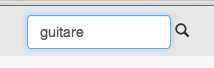
\includegraphics[scale=1]{rechercheWeb}
\caption{Recherche d'une partition ou d'un utilisateur}
\end{figure}

Il est aussi possible d'effectuer des recherches d'utilisateurs et de partitions dans la base de données (à partir du champ recherche du site).
\paragraph{}
Enfin, l'application web est structurée de manière à respecter au mieux certaines conventions établies par la communauté NodeJS. \\
Nous avons donc un dossier config qui contient toutes les informations de configuration de l'application. Ce dossier contient plus particulièrement les fichiers routes.js et sockets.js qui permettent de rediriger vers le bon controller en fonction de l'action à effectuer. \\
De plus, nous avons un dossier controllers qui contient tous les controllers de l'application. Ces controllers contiennent les méthodes à effectuer pour chaque action. Ils utilisent les objets du modèle qui sont définis dans le dossier modèles. \\
Puis le dossier public contient l'application côté client, donc les différentes sources Handlebars qui seront traduites en HTML, le code CSS et le code Javascript de l'application. \\
Chaque dossier contient plusieurs fichiers qui représentent les composants importants de l'application. Par exemple, le dossier modèles contient des fichiers comme user.js ou encore tab.js. De même, le controller qui intéragit avec la partie user se situe dans le dossier controllers et s'intitule user.js (Ceci est une convention de nommage et de structure utilisée par la communauté NodeJS). \\
Enfin, à la racine de l'application il y a le fichier principal pour lancer le serveur: app.js ainsi que différents fichiers de configurations pour des applications telles que Grunt (Gruntfile), Compass (config.rb) ou NodeJS (package.json). \\

\paragraph{}
Au niveau des fonctionnalités implantées, nous avons fait le profil utilisateur ainsi que le profil d'une tablature. Nous n'avons pas eu le temps de faire le profil d'un groupe. La plupart des fonctions du controller et du modèle pour le groupe sont codées mais il manque les différentes vues associées. Certaines vues ne sont pas suffisament travaillées par manque de temps. \\
La page d'accueil du site est une page qui recense les différentes tablatures postées par les personnes que suivent l'utilisateur connecté.
Elle se résume donc à une liste de tablatures que l'on peut télécharger.
Voici un exemple de page du site, la page de profil d'un utilisateur

\begin{figure}[H]
\centering
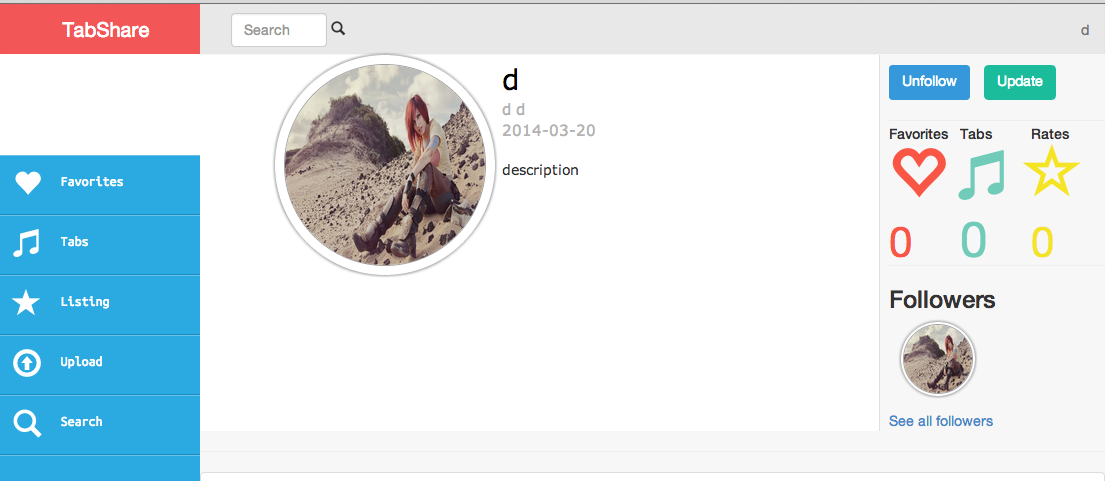
\includegraphics[scale=0.3]{profilUserWeb}
\caption{Page de profil d'un utilisateur}
\end{figure}
\paragraph{}
Pour l'exemple, voici la même page adaptée pour mobile (le site est donc Responsive). Un menu apparait lors d'un clic sur les deux barres noires en haut à gauche, ce qui permet à la page de prendre moins de place en largeur et donc d'être mieux affichée sur un navigateur mobile.
\begin{figure}[H]
\centering
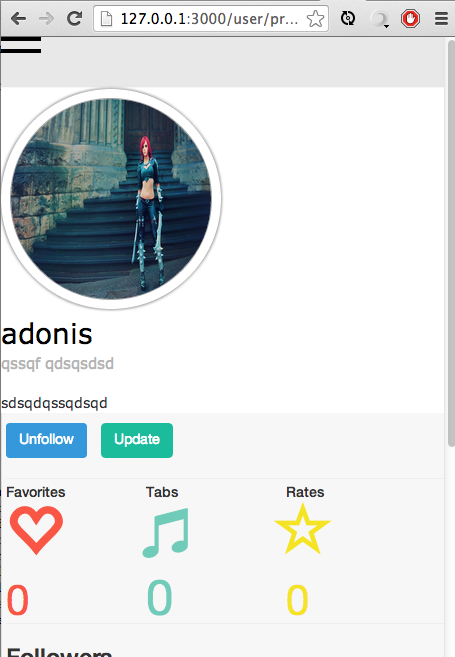
\includegraphics[scale=0.5]{Responsive1}
\caption{Page de profil d'un utilisateur pour mobile}
\end{figure}
\paragraph{}

\paragraph{}
Si on revient sur la version Desktop du site, nous pouvons voir à gauche tout le menu de navigation de l'utilisateur connecté.

\begin{figure}[H]
\centering
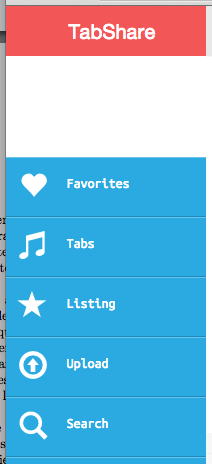
\includegraphics[scale=0.5]{leftWEB}
\caption{Menu de gauche}
\end{figure}

L'affichage des favoris de l'utilisateur connecté se fait en cliquant sur le bouton du même nom (Cette fonction n'est pas implantée pour le moment). De la même manière, le bouton tabs affiche toutes les tablatures que possède l'utilisateur connecté. Enfin, le bouton listing permet quant à lui d'afficher l'ensemble des partitions du site. Le bouton Upload permet d'uploader une nouvelle tablature et le bouton search permet de faire une recherche de tablatures ou d'utilisateurs. L'utilisateur a aussi la possiblité de faire une recherche plus rapide à l'aide de la barre de recherche disponible en haut à gauche. En haut à droite on peut voir le pseudo de l'utilisateur. En cliquant dessus, on a accès à un petit menu qui permet d'avoir un lien vers sa page de profil. \\

\begin{figure}[H]
\centering
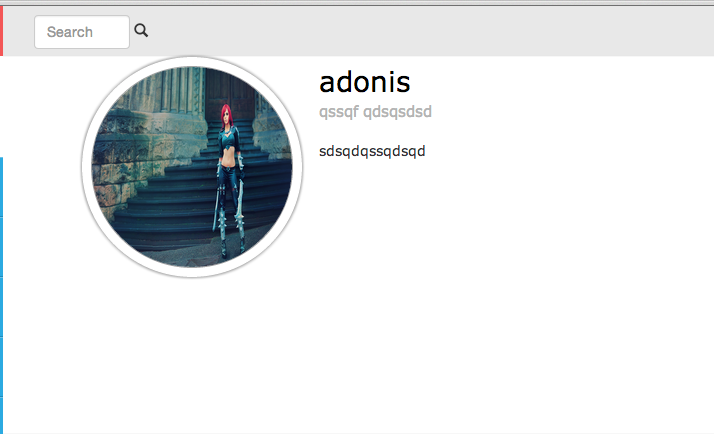
\includegraphics[scale=0.5]{centerWEB}
\caption{Profil de l'utilisateur adonis}
\end{figure}

En ce qui concerne la page de profil en elle-même, nous pouvons voir l'image de profil de l'utilisateur concerné ainsi que différentes informations comme sa description, sa date de naissance ou son prénom. \\

\begin{figure}[H]
\centering
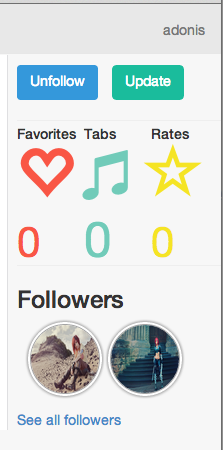
\includegraphics[scale=0.5]{rightWEB}
\caption{Menu de droite}
\end{figure}

Puis, à droite, nous avons des informations sur son activité sur le site, le nombre de tablatures qu'il possède, son nombre de favoris, la note moyenne de toutes les tablatures qu'il a posté et enfin la liste de tous ses followers (les personnes qui ont dans leur fil d'actualité les tablatures qu'il a créées).
